\documentclass[journal,12pt,twocolumn]{IEEEtran}
\usepackage{setspace}
\usepackage{gensymb}
\singlespacing
\usepackage[cmex10]{amsmath}
\usepackage{amsthm}
\usepackage{tcolorbox}
\usepackage{mathrsfs}
\usepackage{txfonts}
\usepackage{stfloats}
\usepackage{bm}
\usepackage{cite}
\usepackage{cases}
\usepackage{subfig}
\usepackage{tasks}
\usepackage{longtable}
\usepackage{multirow}
\usepackage{enumerate}
\usepackage{mathtools}
\usepackage{steinmetz}
\usepackage{tikz}
\usepackage{circuitikz}
\usepackage{verbatim}
\usepackage{tfrupee}
\usepackage[breaklinks=true]{hyperref}
\usepackage{graphicx}
\usepackage{tkz-euclide}
\usetikzlibrary{calc,math}
\usepackage{listings}
    \usepackage{color}                                            %%
    \usepackage{array}                                            %%
    \usepackage{longtable}                                        %%
    \usepackage{calc}                                             %%
    \usepackage{multirow}                                         %%
    \usepackage{hhline}                                           %%
    \usepackage{ifthen}                                           %%
    \usepackage{lscape}     
\usepackage{multicol}
\usepackage{chngcntr}

\DeclareMathOperator*{\Res}{Res}

\renewcommand\thesection{\arabic{section}}
\renewcommand\thesubsection{\thesection.\arabic{subsection}}
\renewcommand\thesubsubsection{\thesubsection.\arabic{subsubsection}}

\renewcommand\thesectiondis{\arabic{section}}
\renewcommand\thesubsectiondis{\thesectiondis.\arabic{subsection}}
\renewcommand\thesubsubsectiondis{\thesubsectiondis.\arabic{sub subsection}}


\hyphenation{optical networks semiconduc-tor}
\def\inputGnumericTable{}                                 %%

\lstset{
%language=C,
frame=single, 
breaklines=true,
columns=fullflexible
}
\begin{document}
\newcommand{\BEQA}{\begin{eqnarray}}
\newcommand{\EEQA}{\end{eqnarray}}
\newcommand{\define}{\stackrel{\triangle}{=}}
\bibliographystyle{IEEEtran}
\raggedbottom
\setlength{\parindent}{0pt}
\providecommand{\mbf}{\mathbf}
\providecommand{\pr}[1]{\ensuremath{\Pr\left(#1\right)}}
\providecommand{\qfunc}[1]{\ensuremath{Q\left(#1\right)}}
\providecommand{\fn}[1]{\ensuremath{f\left(#1\right)}}
\providecommand{\e}[1]{\ensuremath{E\left(#1\right)}}
\providecommand{\sbrak}[1]{\ensuremath{{}\left[#1\right]}}
\providecommand{\lsbrak}[1]{\ensuremath{{}\left[#1\right.}}
\providecommand{\rsbrak}[1]{\ensuremath{{}\left.#1\right]}}
\providecommand{\brak}[1]{\ensuremath{\left(#1\right)}}
\providecommand{\lbrak}[1]{\ensuremath{\left(#1\right.}}
\providecommand{\rbrak}[1]{\ensuremath{\left.#1\right)}}
\providecommand{\cbrak}[1]{\ensuremath{\left\{#1\right\}}}
\providecommand{\lcbrak}[1]{\ensuremath{\left\{#1\right.}}
\providecommand{\rcbrak}[1]{\ensuremath{\left.#1\right\}}}
\theoremstyle{remark}
\newtheorem{rem}{Remark}
\newcommand{\sgn}{\mathop{\mathrm{sgn}}}
\providecommand{\abs}[1]{\vert#1\vert}
\providecommand{\res}[1]{\Res\displaylimits_{#1}} 
\providecommand{\norm}[1]{\lVert#1\rVert}
\providecommand{\mtx}[1]{\mathbf{#1}}
\providecommand{\mean}[1]{E[ #1 ]}
\providecommand{\fourier}{\overset{\mathcal{F}}{ \rightleftharpoons}}
\providecommand{\system}{\overset{\mathcal{H}}{ \longleftrightarrow}}
\newcommand{\solution}{\noindent \textbf{Solution: }}
\newcommand{\cosec}{\,\text{cosec}\,}
\providecommand{\dec}[2]{\ensuremath{\overset{#1}{\underset{#2}{\gtrless}}}}
\newcommand{\myvec}[1]{\ensuremath{\begin{pmatrix}#1\end{pmatrix}}}
\newcommand{\mydet}[1]{\ensuremath{\begin{vmatrix}#1\end{vmatrix}}}
\numberwithin{equation}{subsection}
\makeatletter
\urlstyle{same}
\title{Assignment  }
\author{Harshal Verma\\
AI21MTECH02003}
\date{April 2021}
\maketitle
Download the python code and LaTex code from
\begin{tcolorbox}
Code source: \url{https://github.com/harshal9876/AI5002/blob/main/Assignment_9/Codes/Assignment_9.py} \\
LaTex code :\url{https://github.com/harshal9876/AI5002/blob/main/Assignment_9/Assignment_9.tex}
\end{tcolorbox}
\section{GATE EC 8}

Problem: Consider a dice with the property that the probability of a face with n dots showing up is proportional to n. The probability of the face with three dots showing up is ?
\section{Solution}
Given , $\Pr(N)$ is proportional to n
 where n=\{1, 2, 3, 4, 5, 6\} is random variable. Let the proportionality constant be 'c'.\\
Then $\Pr(N = n) = n \times c $, tabulating the outcomes: 
\begin{center}
\begin{tabular}{ |c | c | c | c | c | c | c |}
\hline
n     & 1 & 2 & 3 & 4 & 5 & 6 \\
\hline
$\Pr(N = n ) = n \times c$ & 1c & 2c&3c &4c & 5c & 6c\\
\hline
\end{tabular}
\end{center}
As the sum of all probability is equal to 1
\begin{align}
\Sigma_{n =1}^6 \Pr(N=n) &= 1\\
c + 2c + 3c + 4c + 5c + 6c &= 1\\
21c &= 1\\
c &= \frac{1}{21}
\end{align}
\text{The probability of three dots showing up is 3c} 
\text{Giving the probability to be:}
\begin{align}
\Pr(N=3) &= 3 \times c\\
&= 3\times\frac{1}{21}\\
&= \frac{3}{21}\\
&= \frac{1}{7}\\
&= 0.1428   
\end{align}
The probability of getting a face with three dots showing up is 0.1428
\begin{figure}[htp]
    \centering
    \captionsetup{justification=centering}
    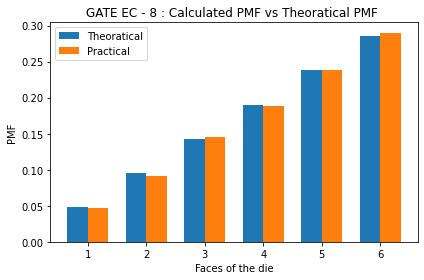
\includegraphics[width=10cm]{Assignment_9_1.png}
    \caption{Calculated PMF versus theoretical PMF}
    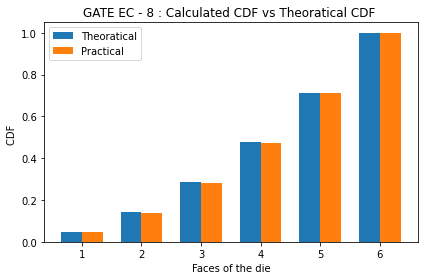
\includegraphics[width=10cm]{Assignment_9_2.png}
    \caption{Calculated CDF versus theoretical CDF}
    \label{fig :plot}
\end{figure}
\vfill
\end{document}
